% FORMATO DEL DOCUMENTO BEAMER A PRESENTAR
\documentclass[a4paper]{article}						% Utilizacion del paquete beamer
	\textheight = 20cm
	\textwidth = 16cm
	\topmargin = -1cm
	\oddsidemargin=0cm
\usepackage[spanish]{babel} 					% Para separar correctamente las palabras
\usepackage{anyfontsize}						%Para cambiar el tamaño de la letra
\usepackage [utf8]{inputenc} 					% Cargamos el modulo de codificacion de caracteres para que acepte tildes y eñes
\usepackage{graphicx}						%Paquete para insertar graficas
\usepackage {currvita}          	%Cargamos el módulo para Curriculum Vitae
\usepackage[dvips]{epsfig}  
\usepackage[T1]{fontenc}
\usepackage[latin1]{inputenc}
\usepackage{tabularx}
\usepackage{url}
\usepackage{pslatex}

\begin{document}

	%CARATULA

	\begin{center}
		\vspace{1cm}
		\textbf{\huge{Escuela Superior Politécnica del Litoral}}\\
		\vspace{0.5cm}
		
\includegraphics[width=5cm]{espol.png} \\
		\vspace{1cm}
		\textbf{\large{Titulo del proyecto}}\\
		\vspace{0.5cm}
		\Large{DRIVE SAFE}\\
		\vspace{1cm}
		\textbf{Asignatura}\\
		\vspace{0.5cm}
		Lenguajes de programacion\\	
		\vspace{1cm}	
		\textbf{\large{Integrantes:}}\\
		\vspace{1cm}
		Marlon Loayza\\
		\vspace{0.3cm}
		Victor Rodriguez\\
		\vspace{0.3cm}
		Carlos Ramirez\\
		\vspace{1cm}
		\textbf{Año Lectivo}\\
		\vspace{0.5cm}
		2012-2013
		\end{center}
		\newpage
	%OBJETIVOS1
	
	\titlepage{\textbf{\Large{OBJETIVOS GENERALES}}}
	\begin{itemize}
		\Large
		\item Aplicar conocimientos necesario, para el desarrollo de la aplicacion en la plataforma movil \textbf{Android}.
		\item Ofrecer una mejora o innovar un recurso para dispositivos \textbf{Android}.
		\item Estimular el trabajo en equipo para la creacion de un software.
		\item Familiarizarnos con la nueva tecnologia, participando en la creacion de ella.
	\end{itemize}
	\newpage
	%INTRODUCCION
	{\parindent=0mm\bf{\Large{Introducción}}}\\
	\vspace{2cm}\\
		\fontsize{14}{0}\selectfont{Con  las nuevas reformas en el reglamento de tránsito y las nuevas forma 
			de sanción que ha implementado la comisión de transito nacional, han surgido muchas irregularidades e inconformidades
			por esta forma de multa por sensores de velocidad, no obstante sin quitarle merito a estas reformas por
			 el decremento de los accidentes de tránsito.}\\
	 \vspace{1cm}\\
		
		\fontsize{14}{0}\selectfont{En base a este problema , surgieron varias necesidades , por ejemplo: }\\
		\vspace{1cm}\\
		\fontsize{14}{0}\selectfont{Como podre evitar ser sancionado cuando este apunto de rebasar un cierto limite 
		de velocidad, en las diferentes zonas de la ciudad?.}\\
		
		\vspace{1cm}\\
		\fontsize{14}{0}\selectfont{Como podre saber si la multa que me marco el sensor que debo pagar, realmente la cometi, tener esta
		informacion de lugar, fecha y hora en que cometi dicha infraccion para asi estar seguro que no es un falso en contra del conductor.}\\
		
		
		\vspace{1cm}\\
		\fontsize{14}{0}\selectfont{En base a estas necesidades hemos implementado nuestro sistema que se explica mas detalladamente
		continuacion en los objetivos especificos y funcionalidad del sistema.}\\
		
	\newpage
	%OBJETIVOS2
	
	\titlepage{\textbf{\Large{OBJETIVOS ESPECIFICOS}}}
	\begin{itemize}
		\Large
		\item Implementar un sistema preventivo de transito.
		\item Prevenir Accidentes causados por exceder limites de velocidad.
		\item Generar un registro de los excesos de velocidad cometidos por alguna emergencia.
		\item Tener un respaldo de nuestras infracciones por limites de velocidad al momento de pagar la multa.
		\item Evitar pagar falsas multas, por una infraccion que nunca cometimos.
	\end{itemize}
	
	\newpage
	%OBJETIVOS2
	
	\titlepage{\textbf{\Large{FUNCIONALIDAD}}}
	  \vspace{1cm}\\
	  \begin{center}
		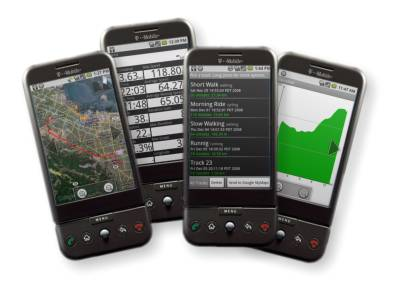
\includegraphics[width=6cm]{funciones.jpg} \\
		\end{center}
		\fontsize{14}{0}\selectfont {Nuestra aplicacion funcionara de la siguiente manera.}\\	
		\vspace{1cm}\\
		\fontsize{14}{0}\selectfont {El usuario activara la aplicacion que se ejecutara en segundo plano.}\\
		\vspace{1cm}\\
		\fontsize{14}{0}\selectfont {Con ayuda del GPS y la alarma de nuestro Smartphone, cuando estemos cerca
		de exceder el limite de velocidad permitido en respectivas zonas como carretera, perimetral, zonas residenciales,
		escuelas hospitales,etc. Nuestro Smartphone lanzara una alarma que nos indica que estamos a punto de exceder el limite
		de velocidad permitido , lanzando una alarma personalizada de precaucion.}\\	
		\begin{center}
		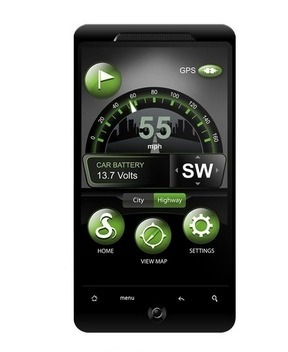
\includegraphics[width=4cm]{velocidad.jpg} \\
		\end{center}
		\newpage
		\fontsize{14}{0}\selectfont {En caso de ignorar esta alarma el Smartphone nos indicara que hemos excedido el limite,
		y nos advertira que hemos cometido una infraccion, guardando la fecha, hora y lugar en que la cometimos.}\\		
		\vspace{1cm}\\
		\begin{center}
		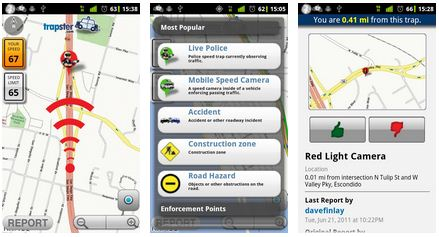
\includegraphics[width=8cm]{registro.jpg} \\
		\end{center}
		\vspace{1cm}\\
		\fontsize{14}{0}\selectfont {De esta manera tenemos un sistema preventivo y a la vez un sistema de control
		que nos respalda al momento de pagar nuestras multas en la comision de transito.}\\	
		\vspace{1cm}\\
		\fontsize{14}{0}\selectfont {Identificación de los radares, para evitar exceder la velocidad en presencia de ellos.}\\
		\vspace{1cm}\\
		\begin{center}
		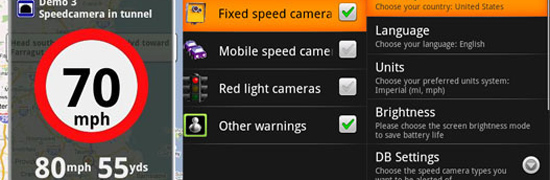
\includegraphics[width=7cm]{radares.jpg} \\
		\end{center}
\end{document}